%%%%%%%%%%%%%%%%%%%%%%%%%%%%%%%%%%%%%%%%%%%%%%%%%%%%%%%%%%%%%%%%%%%%%%%%%%%%%%%%
% AMS Beamer series / Bologna FC / Template
% Andrea Omicini
% Alma Mater Studiorum - Università di Bologna
% mailto:andrea.omicini@unibo.it
%%%%%%%%%%%%%%%%%%%%%%%%%%%%%%%%%%%%%%%%%%%%%%%%%%%%%%%%%%%%%%%%%%%%%%%%%%%%%%%%
%\documentclass[handout]{beamer}\mode<handout>{\usetheme{default}}
%
\documentclass[presentation]{beamer}\mode<presentation>{\usetheme{AMSBolognaFC}}
%\documentclass[handout]{beamer}\mode<handout>{\usetheme{AMSBolognaFC}}
%%%%%%%%%%%%%%%%%%%%%%%%%%%%%%%%%%%%%%%%%%%%%%%%%%%%%%%%%%%%%%%%%%%%%%%%%%%%%%%%
\usepackage[T1]{fontenc}
\usepackage{wasysym}
\usepackage{amsmath,blkarray}
\usepackage{centernot}
\usepackage{fontawesome}
\usepackage{fancyvrb}
\usepackage[ddmmyyyy]{datetime}
\renewcommand{\dateseparator}{}
%\renewcommand{\thefootnote}{\fnsymbol{footnote}}
\newcommand{\version}{1}
\usepackage[
	backend=biber,
	citestyle=authoryear-icomp,
	maxcitenames=1,
	bibstyle=alphabetic]{biblatex}

	\makeatletter

\addbibresource{biblio.bib}
%%%%%%%%%%%%%%%%%%%%%%%%%%%%%%%%%%%%%%%%%%%%%%%%%%%%%%%%%%%%%%%%%%%%%%%%%%%%%%%%
\title[On Collective Reinforcement Learning]
{On Collective Reinforcement Learning}
%
\subtitle[Techniques, Challenges, and Opportunities]
{Techniques, Challenges, and Opportunities}
%
\author[\sspeaker{Aguzzi}]
{\speaker{Gianluca Aguzzi} \href{mailto:gianluca.aguzzi@unibo.it}{gianluca.aguzzi@unibo.it}}
%
\institute[DISI, Univ.\ Bologna]
{Dipartimento di Informatica -- Scienza e Ingegneria (DISI)\\\textsc{Alma Mater Studiorum} -- Universit{\`a} di Bologna}
%
\renewcommand{\dateseparator}{/}
\date[\today]{\today}
%
%%%%%%%%%%%%%%%%%%%%%%%%%%%%%%%%%%%%%%%%%%%%%%%%%%%%%%%%%%%%%%%%%%%%%%%%%%%%%%%%
\begin{document}
%%%%%%%%%%%%%%%%%%%%%%%%%%%%%%%%%%%%%%%%%%%%%%%%%%%%%%%%%%%%%%%%%%%%%%%%%%%%%%%%

%/////////
\frame{\titlepage}
%/////////

%%===============================================================================
\section*{Outline}
%%===============================================================================

%%/////////
\frame[c]{\tableofcontents[hideallsubsections]}
%%/////////

%===============================================================================
\section{Introduction}
%===============================================================================

%/////////
\begin{frame}[c]{Introduction}
%/////////
\begin{alertblock}{Motivation}
	\begin{itemize}
		\item Learning is a key mechanism to drive \emph{adaptivity}
		\item Intelligent agents improve their performance with \emph{experience}
		\item We would like to improve adaptiveness with raw experience and, hence 
		\item We would like to bring Reinforcement Learning methodology in CAS
	\end{itemize}
\end{alertblock}
\begin{alertblock}{Lecture goals}
	\begin{itemize}
		\item Understanding the challenges related to the Multi-Agent System (MAS) domain
		\item Show Techniques, Patterns, and Architecture applied in \emph{Collective} Systems
		\item Hands-on in some practical example of \emph{Collective} Learning
	\end{itemize}
\end{alertblock}
%
\end{frame}
%/////////

%/////////
\begin{frame}[c, fragile]{Single-Agent Learning}
%/////////
\begin{exampleblock}{What have you seen so far \dots}
	\begin{itemize}
		\item Markov Decision Process (MDP) to model the agent-environment interactions
		\item Find a learning process that eventually leads to an \emph{optimal} policy $\pi^*$
		\item Q-Learning (in general \emph{value-based approaches}) as a prominent algorithm to reach converge
	\end{itemize}
\end{exampleblock}
\begin{alertblock}{\dots But plain RL works only under some conditions}
	\begin{itemize}
		\item Reward hypothesis
		\item Full environment observability and Markovian property
		\item Stationary environment
		\item State/action space should be small enough to be stored in memory (otherwise, we should leverage function approximators)
	\end{itemize}	
\end{alertblock}
\end{frame}
%/////////
\begin{frame}{Partial Observable environments}
%/////////
	\begin{alertblock}{Definition}
		An agent does not have a \emph{perfect} and \emph{complete} knowledge of the state of the environment
	\end{alertblock}

	\begin{figure}
		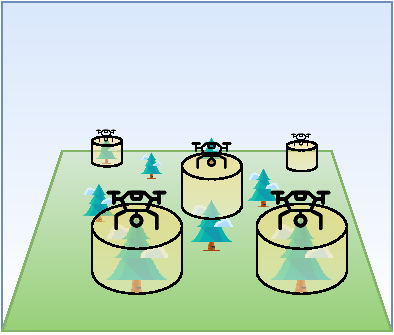
\includegraphics[height=5cm]{img/challenge-partial-observable.pdf}
	\end{figure}
\end{frame}

%\begin{frame}{Partial Observable Environments}
%	\begin{exampleblock}{Partial Observable MDP $\mathcal{P}$ (POMDP) \href{https://www.pomdp.org/}{\faLink}}
%		\begin{itemize}
%			\item An agent cannot directly observe the system state, but he can make \emph{observations} that depend on this state
%			\item POMDP is a tuple $(S, A, T, R, \Omega, O)$
%			\item $S, A, T, R$ are the same variable described in MDP
%			\item $\Omega$ is the set of observations perceived by the agent $\{o_1, \dots, o_n\}$
%			\item $O$ is the set of conditional probability $O(o | s, a)$
%			\item I want to learn a policy that depends on $o$ but that maximises a reward function that depends on $s$
%			\item The agents need to build a belief state from the history of the observations
%		\end{itemize}
%	\end{exampleblock}
%\end{frame}
%/////////
\begin{frame}[c]{Non-stationary environments}
%/////////
	\begin{alertblock}{Definition}
		The environment model (e.g. the random variable associated with it) changes
		over time.
	\end{alertblock}
	\begin{exampleblock}{MDP are Stationary by definition \dots}
		\begin{itemize}
			\item \dots But, real-case environment dynamics could change over time (e.g. markets, city traffic, routing networks)
			\item Practically, it seems that RL (in particular Temporal Difference (TD) methods) works well even in this case
			\item \emph{But, we lose convergence guarantees.}
		\end{itemize}
	\end{exampleblock}
%
\end{frame}

%===============================================================================
\section{From Single Agent To Multi-Agent}
%===============================================================================

%/////////
\begin{frame}[c]{From Single-Agent To Multi-Agent}
%/////////
	\begin{alertblock}{Multi-Agent Reinforcement Learning (MARL)}
		\centering
		\emph{Multiple agents learn \textbf{together} the best policy that maximises
	a long term reward signal.}
	\end{alertblock}
	\begin{exampleblock}{Considerations}
		\begin{itemize}
			\item If multiple agents exist, but only \textbf{one} agent learns by experience, then it is a single agent problem (e.g. single-player videogames)
			\item So, MAS + Learning $\centernot\implies$ MARL, \textbf{but} MARL $\implies$ MAS
		\end{itemize}
	\end{exampleblock}
	\begin{columns}
		\begin{column}{0.4\textwidth}
			\raggedleft
			\begin{figure}
				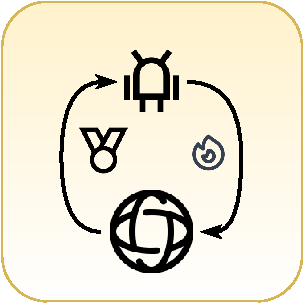
\includegraphics[height=2.5cm]{img/single-agent-multi-agent-1.pdf}
			\end{figure}
		\end{column}
		\begin{column}{0.4\textwidth}	
			\raggedright
			\begin{figure}
				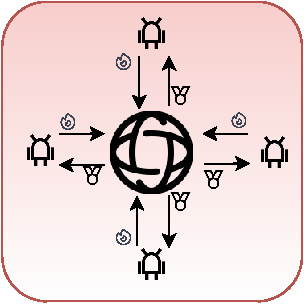
\includegraphics[height=2.5cm]{img/single-agent-multi-agent-2.pdf}
			\end{figure}
		\end{column}
	\end{columns}
\end{frame}
%/////////
\begin{frame}[c]{Stochastic Game $\mathcal{S}$ (or Markov games)}
%/////////
	\begin{alertblock}{}
		\begin{itemize}
			\item Extension of MDP to the MAS context
			\item Common abstraction in MARL algorithms
		\end{itemize}
	\end{alertblock}
	\begin{alertblock}{Definition}
		\begin{itemize}
			\item $\mathcal{S}$ is a tuple $<N, S, \{A^i\}_{i \in \{ 1, \dots, N\}}, P, \{R^i\}_{i \in \{ 1, \dots, N\}}>$
			\item $N$ is the number of agents ($|N| > 1 $)
			\item $S$ is the global environment state
			\item $A^i$ is the action state of agent $i$. $\mathbb{A} := A^1 \times \dots\times A^N$ is the joint action space
			\item $P: S x \mathbb{A} \rightarrow \mathcal{P}(S)$ is the state transaction. $\mathcal{P}$ is a discrete probabilistic distribution (associate for each $s \in S$ a probability)
			\item $R^i: S \times \mathbb{A} \times S \rightarrow \mathbb{R}$ is the reward signal
			\item Typical time evolution: $ S_0, \mathbb{A}_0, \mathbb{R}_1, S_1, \dots  $
		\end{itemize}
	\end{alertblock}
\end{frame}
%/////////
\begin{frame}[fragile]{Stochastic games: Example}
%/////////
	\begin{exampleblock}{Paper Rock Scissor}
		\begin{itemize}
			\item $N = 2$
			\item $A^1 = A^2 = $ \{Paper, Rock, Scissor\}
			\item $S = $ \{ \}
			\item $R = \begin{blockarray}{cccc}
        & Rock & Paper & Scissor \\
      \begin{block}{c[ccc]}
        Rock    & 0, 0  & -1, 1 & 1, -1 \\
        Paper   & 1, -1 & 0, 0  & -1, 1 \\
        Scissor & -1, 1 & 1, -1 & 0, 0 \\
      \end{block}
    \end{blockarray}$
		\end{itemize}
	\end{exampleblock}
\end{frame}
%/////////
\begin{frame}{MARL Systems: Task type}
%/////////
	\begin{alertblock}{Cooperative}
		\begin{itemize}
			\item Agents share the same reward function ($R^1 = \dots = R^N$) in order to accomplish a collective goal
		\end{itemize}
	\end{alertblock}
	\begin{figure}
		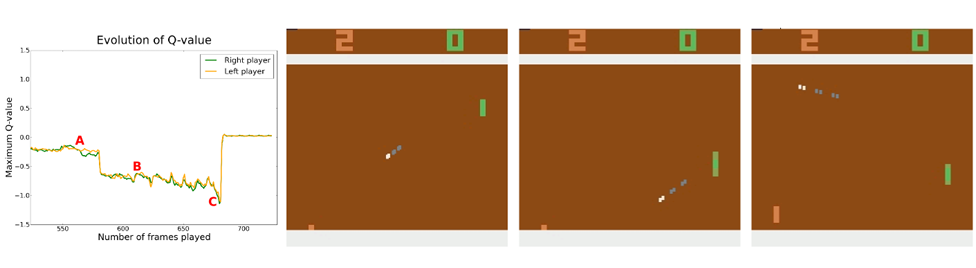
\includegraphics[height=5cm]{img/cooperative}
	\end{figure}
\end{frame}

\begin{frame}{MARL Systems: Task type}
	\begin{exampleblock}{Competitive}
		\begin{itemize}
			\item Agents compete with each other to maximise a long term return
			\item Board Games, Video games, \dots
		\end{itemize}
	\end{exampleblock}

	\begin{figure}
		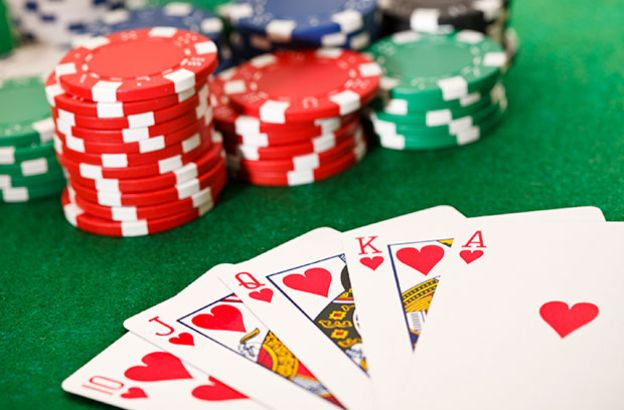
\includegraphics[height=5cm]{img/competitive}
	\end{figure}
\end{frame}

\begin{frame}{MARL Systems: Task type}
	\begin{exampleblock}{Mixed}
		\begin{itemize}
			\item Agents can both compete and cooperate in order to maximise a global reward function
			\item Also called \textit{General Sum games}
		\end{itemize}
	\end{exampleblock}

	\begin{figure}
		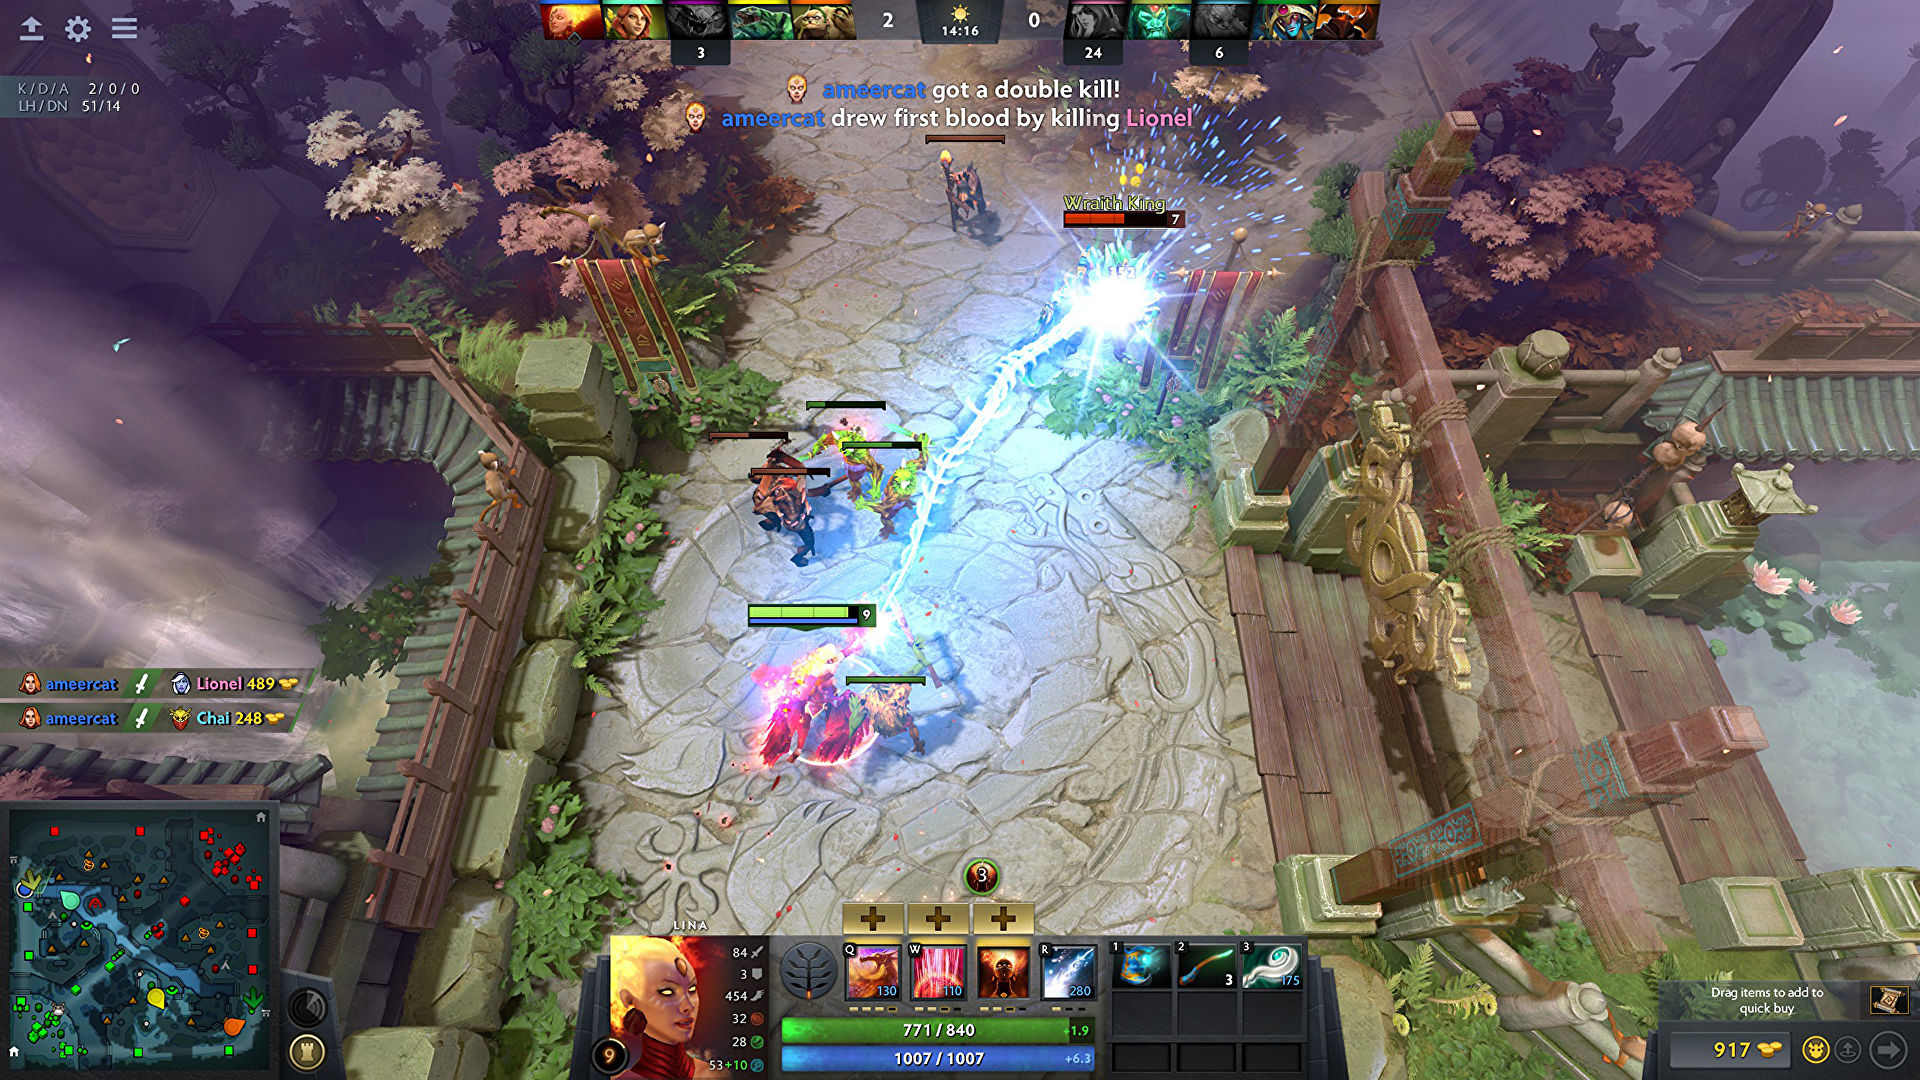
\includegraphics[height=5cm]{img/mixed}
	\end{figure}
\end{frame}

\begin{frame}{On Cooperative Task}
	\begin{exampleblock}{Homogeneous}
		\begin{itemize}
			\item Each agent has same capabilities ($A^1 = \dots = A^N$)
			\item The overall goal is to find the best policy that is the same for each agent ($\pi^* = {\pi^{*}}_1 = \pi^{*}_2 = \dots = {\pi^{*}}_N$)
		\end{itemize}
	\end{exampleblock}
	\begin{exampleblock}{Heterogeneous}
		\begin{itemize}
			\item Each agent could have different capabilities (in the worst case, $A^1 \neq \dots \neq A^N$)
			\item Each agent has its local policy that should be maximised following the global collective goal
		\end{itemize}
	\end{exampleblock}
\end{frame}

%/////////
\begin{frame}{MARL Systems: Learning Scheme}
	\begin{exampleblock}{Centralised Training and Centralised Execution (CTCE)}
		\begin{itemize}
			\item \emph{One} agent with a global view of the system (in the cloud? in a server?)
			\item Nodes send their perception to that central agent
			\item With this perceptions, it creates a global state of the system
			\item With the current policy, it chooses the actions that nodes should performance (\emph{Control})
			\item In the next time step, it evaluates the reward function and updates the policy accordingly (\emph{Learn})
			\item \emph{Are the nodes agents?}
			\item Used mainly in offline (i.e. at simulation time) setting 
		\end{itemize}
	\end{exampleblock}

\end{frame}
%/////////

%/////////
\begin{frame}{MARL Systems: Learning Scheme}
	\begin{exampleblock}{Centralised Training and Centralised Execution (CTCE)}
		\begin{figure}
			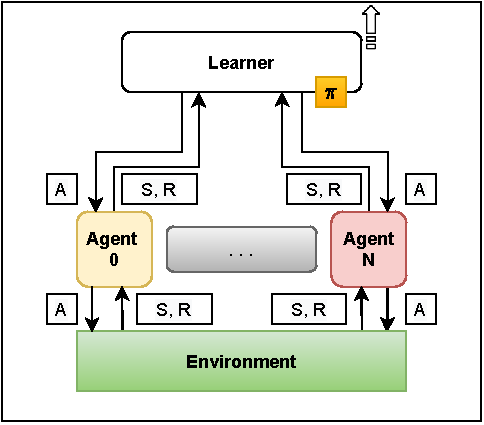
\includegraphics[height=6cm]{img/learning-scheme-clce.pdf}
		\end{figure}
	\end{exampleblock}
\end{frame}
%/////////

%/////////
\begin{frame}{MARL Systems: Learning Scheme}
	
	\begin{exampleblock}{Decentralised Training and Decentralised Execution (DTDE)}
		\begin{itemize}
			\item Each node has its local policy/value table
			\item They can perceive the environment state (or they can observe a part of it)
			\item With the current state, they perform an action following their local policy (\emph{Control})
			\item In the next time step, they update their policy following a local reward function (\emph{Learn})
			\item Both used in offline and online (i.e. deployment time) setting
		\end{itemize}
	\end{exampleblock}
\end{frame}
%/////////


%/////////
\begin{frame}{MARL Systems: Learning Scheme}
	\begin{exampleblock}{Decentralised Training and Decentralised Execution (DTDE)}
		\begin{figure}
			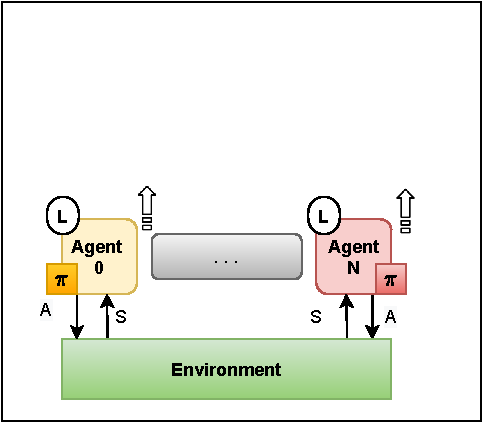
\includegraphics[height=6cm]{img/learning-scheme-dtde.pdf}
		\end{figure}
	\end{exampleblock}
\end{frame}

\begin{frame}{MARL Systems: Learning Scheme}
	
	\begin{exampleblock}{Centralised Training and Decentralised Execution (CTDE)}
		\begin{itemize}
			\item A simulation time learning online execution pattern
			\item \emph{Simulation time}
			\begin{itemize}
				\item Each node follows the typical $o_t, a_t, o_{t+1}, a_{t+1},\dots $ trajectory using a local policy
				\item After an episode, this trajectory (or something derived from it) will be sent to a central learner
				\item It, using a global view of the system, improves the policies of the agents 
				\item An then the policies will be shared with the agents
			\end{itemize} 
			\item \emph{Execution time}
				\begin{itemize}
					\item Each agent has the local policy distilled during the simulation time
					\item With it, they act in the environment
				\end{itemize}
		\end{itemize}
	\end{exampleblock}
\end{frame}


\begin{frame}{MARL Systems: Learning Scheme}
	\begin{exampleblock}{Decentralised Training and Decentralised Execution (DTDE)}
		\begin{figure}
			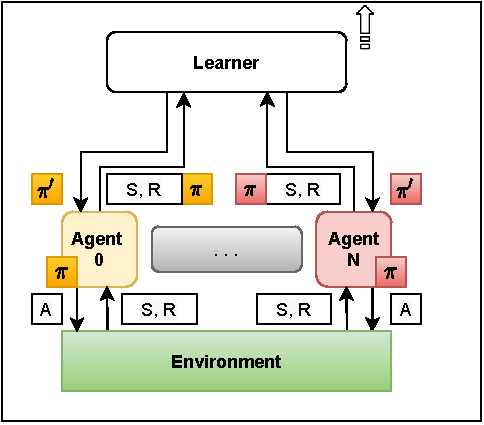
\includegraphics[height=6cm]{img/learning-scheme-ctde.pdf}
		\end{figure}
	\end{exampleblock}
\end{frame}

\begin{frame}{MARL Systems: Successful Applications}
	\centering
	\begin{exampleblock}{OpenAI Hide And Seek: \url{https://openai.com/blog/emergent-tool-use/}}
		\begin{figure}
			\href{https://www.youtube.com/watch?v=kopoLzvh5jY}{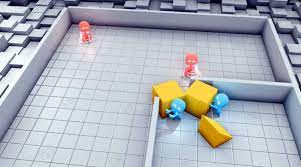
\includegraphics{img/hide-and-seek.jpeg}}
		\end{figure}
	\end{exampleblock}
\end{frame}

\begin{frame}{MARL Systems: Successful Applications}
	
	\begin{exampleblock}{Capture The Flag: \url{https://deepmind.com/blog/article/capture-the-flag-science}}
	\begin{figure}
		\centering
		\href{https://www.youtube.com/watch?v=dltN4MxV1RI}{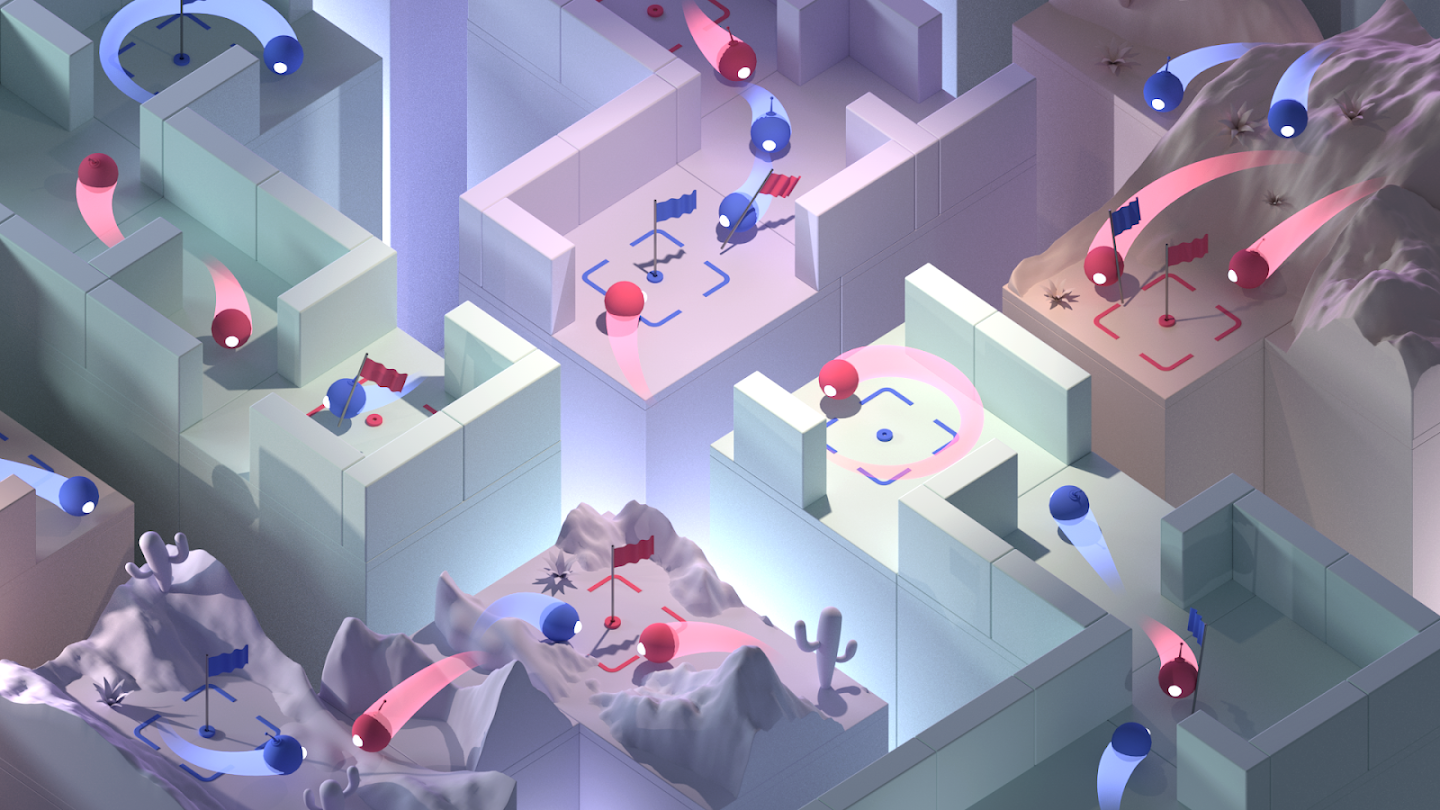
\includegraphics[width=0.85\textwidth]{img/capture-the-flag.png}}
	\end{figure}	
	\end{exampleblock}
\end{frame}
%===============================================================================
\section{Learning in CAS}

\begin{frame}{Collective Adaptive System (CAS)}
	\begin{alertblock}{Recap}
		Systems composed by a (possibly) large set of components executing a \emph{collective} task relying on component interactions and showing \emph{inherent} adaptiveness. 
	\end{alertblock}
	\begin{columns}
		\begin{column}{0.5\textwidth}		
			\begin{figure}
				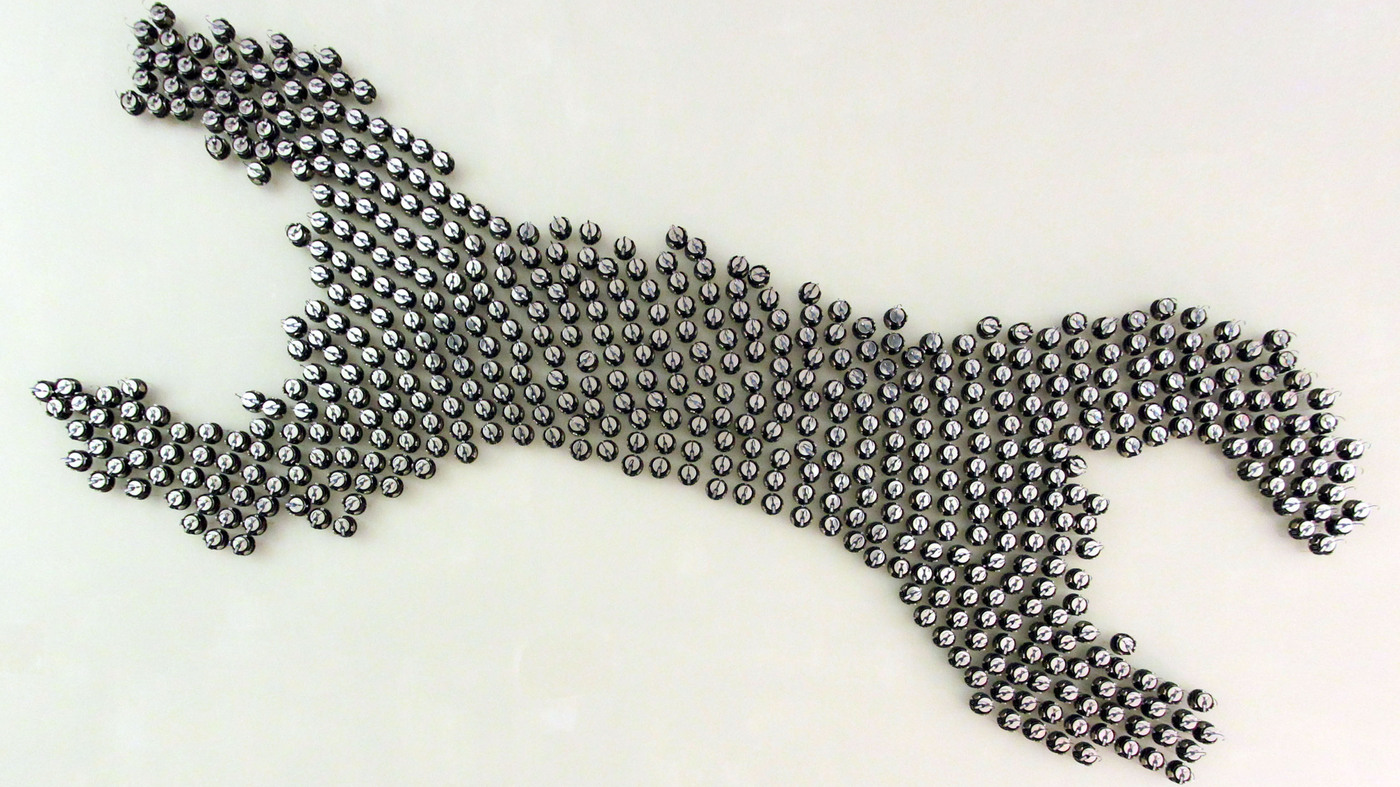
\includegraphics[height=3cm]{img/cas-1}
			\end{figure}
		\end{column}
	

		\begin{column}{0.5\textwidth}	
			\begin{figure}
				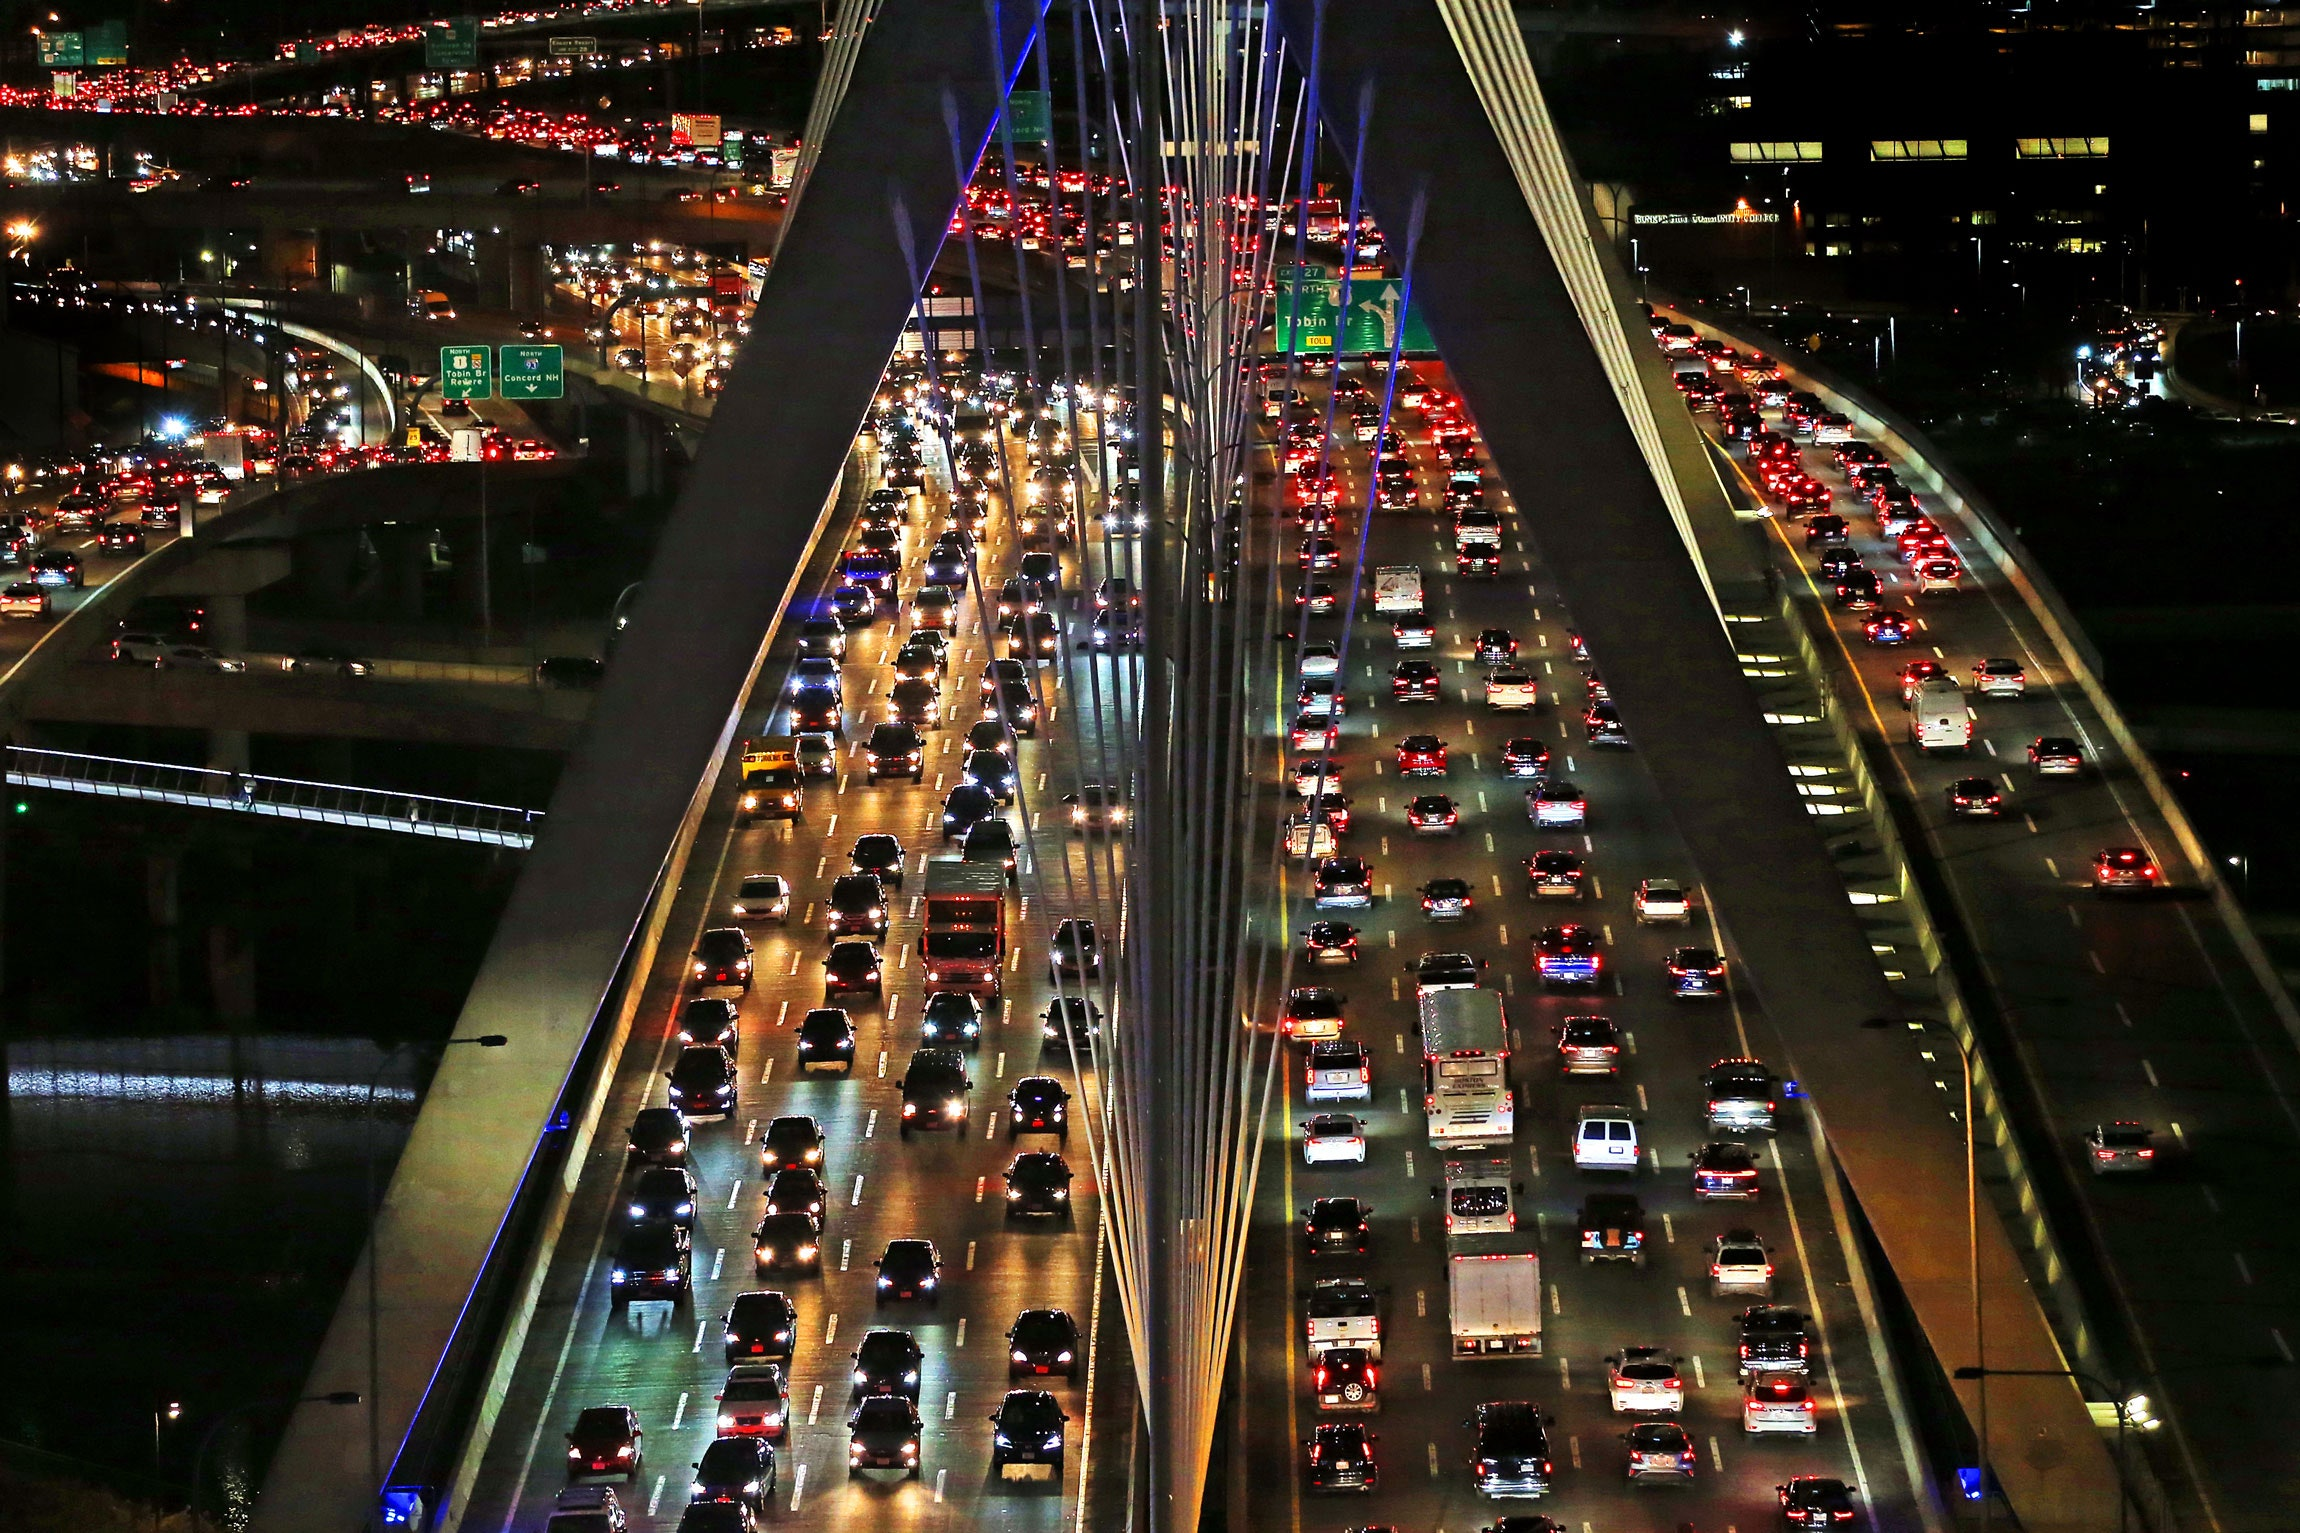
\includegraphics[height=3cm]{img/cas-3}
			\end{figure}
		\end{column}
	\end{columns}
\end{frame}
%===============================================================================
\begin{frame}[c]{Learning in CAS~\footnote[frame]{\fullcite{DBLP:conf/icse/DAngeloGGGNPT19}}}
\begin{exampleblock}{Constraints}
	\begin{itemize}
		\item The collective goal could be accomplished through competition and/or cooperation 
		\item The system could be heterogeneous or homogeneous
		\item The agent number is not bounded (openness)
		\item Distributed control -- i.e. no central authority exists
	\end{itemize}
\end{exampleblock}
\end{frame}
%/////////
\begin{frame}[c]{Learning in CAS: Challenges}
	\begin{exampleblock}{CASs are partial observable}
		Each agent could only perceive a part of the system through its sensors.
	\end{exampleblock}
	\begin{alertblock}{Learning in CASs make the environments non-stationary}
		Each agent learns concurrently $\implies$ by the eye of an agent the environment is in continuous evolution.
	\end{alertblock}
	\begin{alertblock}{The curse of dimensionality -- MAS combinatorial nature}
		When we have to deal with a large number of agents, the overall state-action space is increasing exponentially to the number of agents --- so a central learner cannot solve the learning problem.
	\end{alertblock}
\end{frame}
%/////////
\begin{frame}[c]{Learning in CAS: Challenges}
	\begin{exampleblock}{Multi-Agent credit assignment problem}
		Typically, in CAS, a global reward function exists. But it is hard to understand the influence of a single agent to
		the overall collective behaviour.
	\end{exampleblock}
	\begin{exampleblock}{Sample efficiency}
		Action-space and state-space are very large in CASs $\implies$ the problem of sample efficiency (i.e. how many samples does the RL need to reach a good policy?)
		arise as in the Deep Learning context. 
	\end{exampleblock}
\end{frame}

\begin{frame}{On sample efficiency: Example of learning time }
	\begin{exampleblock}{A Nowadays problem \dots}
		\begin{itemize}
			\item Nowadays, Deep Learning Techniques are used to train complex neural networks
			\item When applied to Reinforcement Learning, the training phase requires millions of interactions for an agent to learn
			\item In the Multi-Agent Setting is even worst \dots
			\item In the previous example\footnote[frame]{\fullcite{DBLP:journals/corr/abs-1807-01281}}, they train 30 agents in 450k games!
		\end{itemize}
	\end{exampleblock}
\end{frame}
\begin{frame}{On scalability: Single Agent Learner Example}
	\begin{exampleblock}{Learning setting}
		\begin{itemize}
			\item A central agent (i.e. in the cloud? In a server?) sees the entire system
			\item Standard RL algorithm (tabular) create a table with the size of $|S \times A|$
			\item But the system-wide action space is the cartesian product of the agent action-space, so the A cardinality is $|A|^N$
			\item With 100 agents with 10 possible actions, we have already reached an action space with more actions then the particles in the universe ($\sim 10^{80}$ \href{https://en.wikipedia.org/wiki/Eddington_number}{\faLink}).
		\end{itemize}
	\end{exampleblock}
\end{frame}
\begin{frame}{Learning in CAS: A Motivating Example}
	\begin{exampleblock}{Robot Collision Avoidance~\footnote[frame]{\fullcite{DBLP:conf/icra/LongFLLZP18}} \url{https://sites.google.com/view/drlmaca}}
		\centering
		\begin{figure}
			\href{https://www.youtube.com/watch?v=Uj1yAmlL5lk}{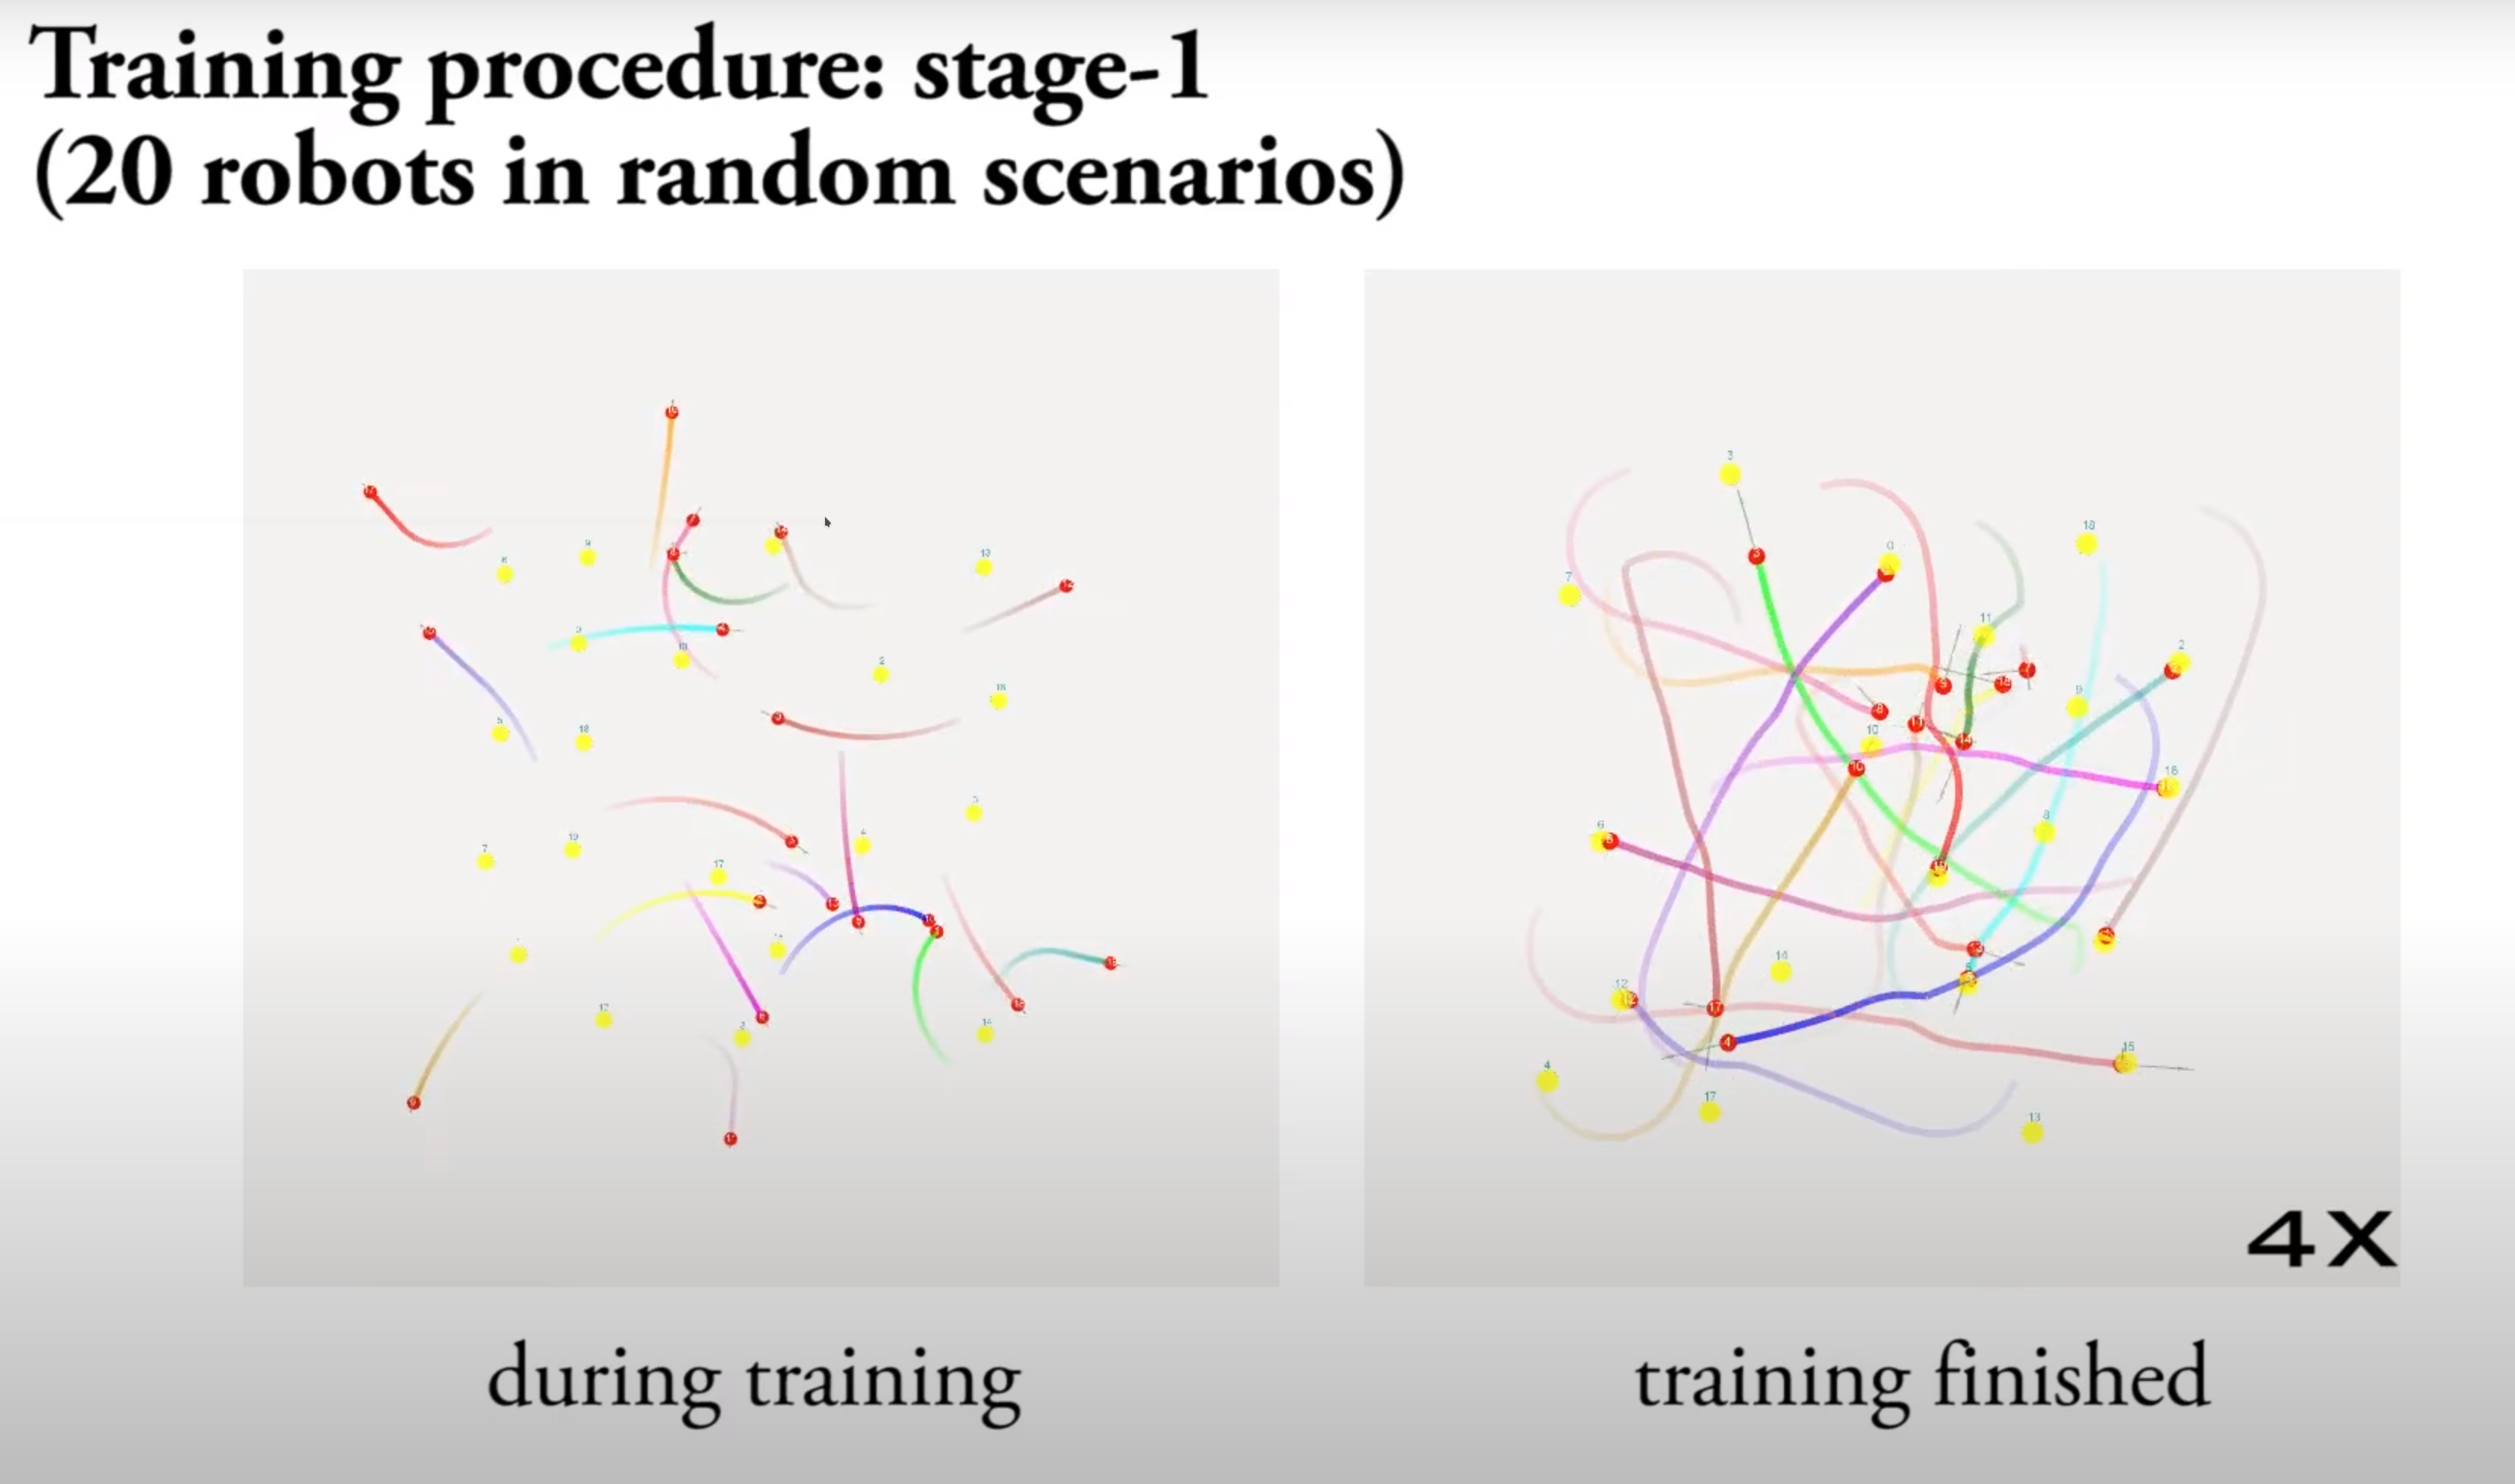
\includegraphics[width=0.7\textwidth]{img/collective-learning.png}}
		\end{figure}
	\end{exampleblock}
\end{frame}
\begin{frame}{Learning in CAS: Toolkits}
	\begin{exampleblock}{MAgent~\footnote[frame]{\fullcite{zheng2018magent}} \url{https://github.com/geek-ai/MAgent}}
		\begin{figure}
			\href{https://www.youtube.com/watch?v=HCSm0kVolqI}{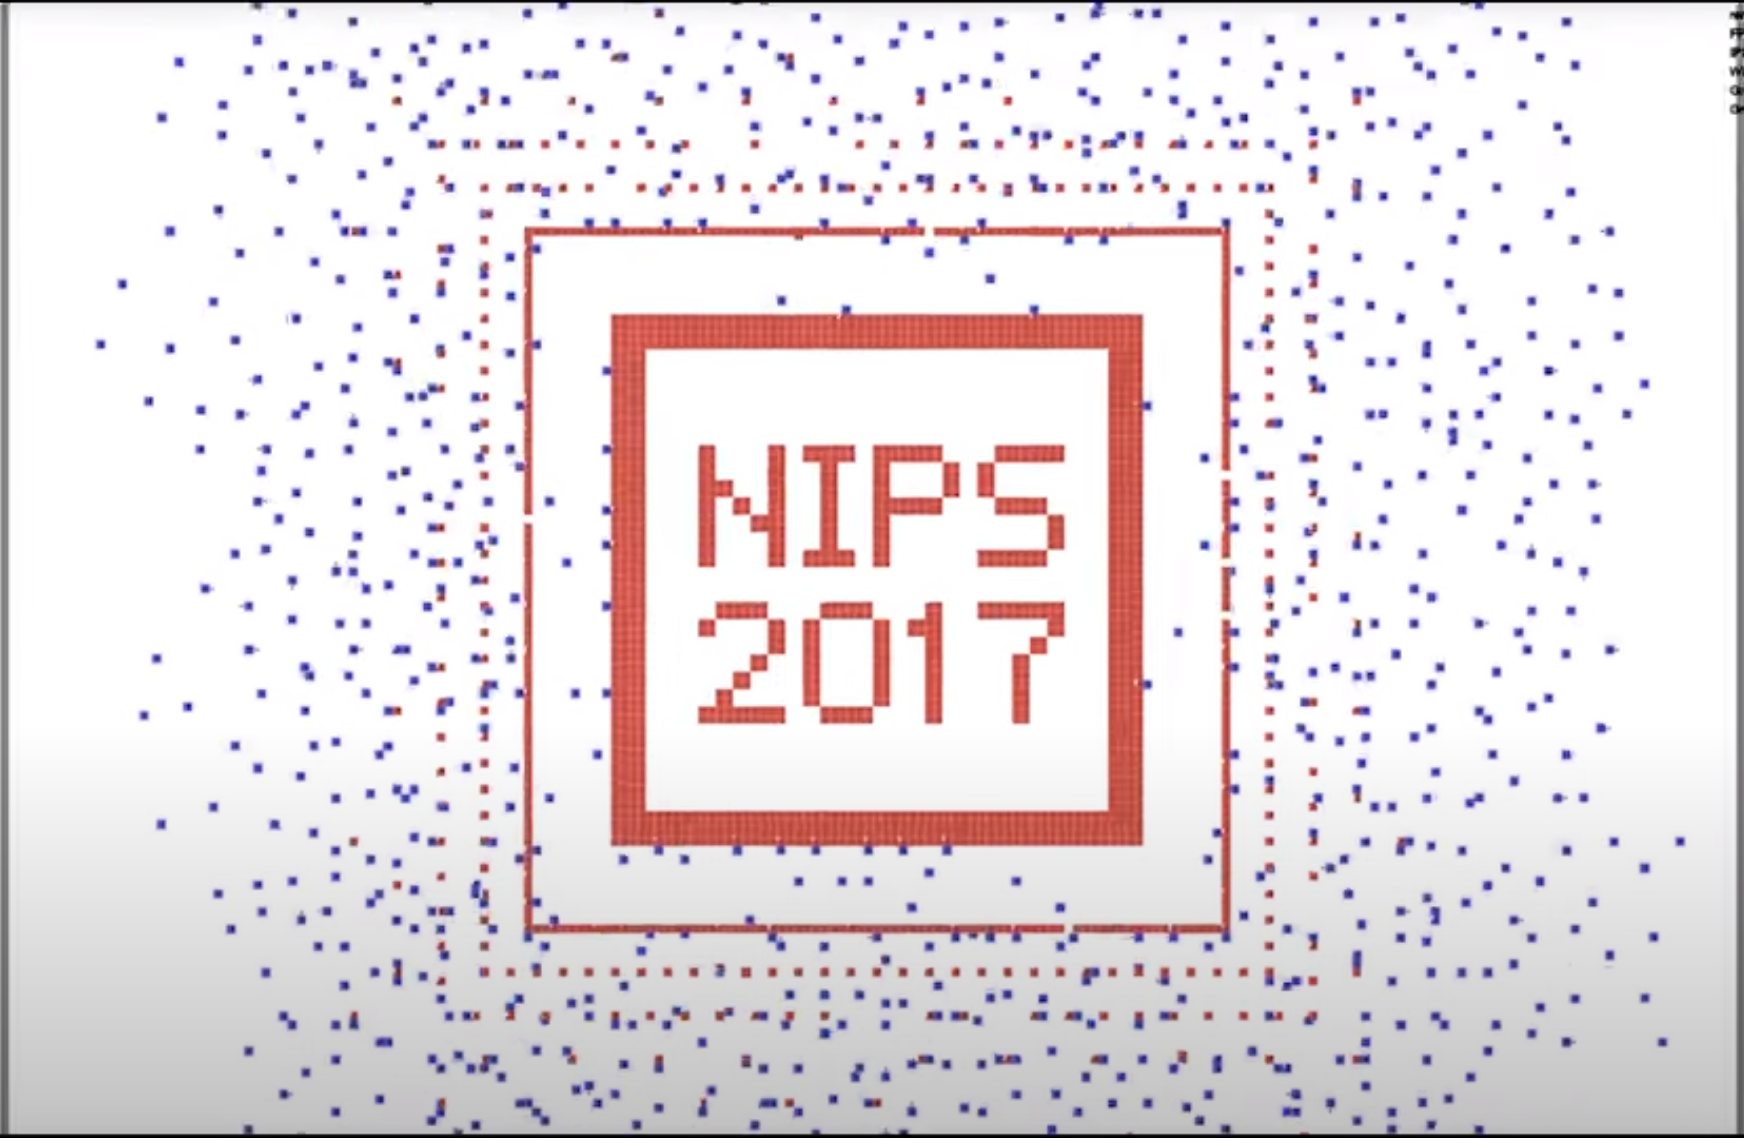
\includegraphics[width=0.7\textwidth]{img/magent.png}}
		\end{figure}
	\end{exampleblock}
\end{frame}
%/////////
\begin{frame}{Learning in CAS: Our today focus}
	\begin{alertblock}{Constraints}
		\begin{itemize}
			\item Learning in cooperative systems: i.e. each entity shares the same reward functions
			\item Learning in homogeneous systems: i.e. each entity is interchangeable with each other
			\item[\faExclamationTriangle] We do not consider partial observability as a core problem
		\end{itemize}
	\end{alertblock}
	\begin{exampleblock}{Homogenous system: Implications}
		\begin{itemize}
			\item[{\color{teal}\faThumbsUp}] The optimal policy is the same for the whole system
			\item[{\color{teal}\faThumbsUp}] During the learning phases, the system can use different policies (e.g. to reduce sample efficiency)
			\item[{\color{teal}\faThumbsUp}] We reduce the action space
			\item[{\color{teal}\faThumbsUp}] We reduce the non-stationarity problem
		\end{itemize}
	\end{exampleblock}
\end{frame}

%\begin{frame}{Learning in CAS: Models}
		
	%\begin{exampleblock}{Dec-POMDP $\mathcal{D}$ \href{http://rbr.cs.umass.edu/camato/decpomdp/overview.html}{\faLink}}
	%	\begin{itemize}
	%		\item Combination of Stochastic games and POMDP
	%		\item $\mathcal{D}$ is a tuple $(N, S, \{A^i\}, P, \{R^i\}, \{{\Omega^{i}}\}O)$
	%		\item For brevity, $\{ \mathfrak{X}^i\} = \{\mathfrak{X}^i\}_{i \in \{1, \dots, N\}}$
	%		\item $N, S, \{A^i\}, P, \{R^i\}$ are the same variables defined in Stochastic games
	%		\item $\{\Omega^{i}\}$ is the same variable defined for POMDP
	%		\item ${\Omega} = \{\Omega^1 \dots \Omega^N \}$  is the joint observation space
	%		\item $O: \mathbb{A} \times S \rightarrow \mathcal{P}(\Omega) $ is the global observation function
	%	\end{itemize}
	%\end{exampleblock}
	%\begin{exampleblock}{Problems}
	%	\begin{itemize}
	%		\item The homogeneity is not captured by the model (different action, observation, and reward spaces)
	%	\end{itemize}
	%\end{exampleblock}
	%\begin{exampleblock}{Dec-POMDP \href{http://rbr.cs.umass.edu/camato/decpomdp/overview.html}{\faLink}}
	%	\begin{itemize}
	%		\item Extension of POMDP to Multi-Agent settings
	%		\item N agent act in a Markovian environment \emph{but} they perceive only partial information about it (observations)
	%		\item[\faExclamationTriangle] Does not consider homogeneity
	%	\end{itemize}
	%\end{exampleblock}
	%\begin{exampleblock}{SwarMDP~\footnote[frame]{\fullcite{DBLP:journals/corr/SosicKZK16}}}
	%	\begin{itemize}
	%		\item Consider a homogeneous population of agents (i.e. same action, observation space and same policy)
	%		\item Learning lead to a single policy that map observation (not history) to action
	%		\item[\faExclamationTriangle] Time continuing to be synchronous
	%	\end{itemize}
	%\end{exampleblock}
%\end{frame}

\begin{frame}{Learning in CAS: A simplified model}
	\begin{exampleblock}{}		
		\begin{itemize}
			\item Each agent is seen as a tuple $(M, \mathcal{N})$
			\item $M$ is a local Markov decision process ($S$ is an observation space in common with the entire system)
			\item $\mathcal{N}$ is the neighbourhood perceived by an agents
			\item The global state system state is unknown
			\item Agents want to learn a policy $\pi(a | s, \mathcal{N})$ to share with the entire system
			\item When agents do not consider neighbours, we call the system as \emph{Independent learners}
			\item When agents consider neighbours actions to choose their local action, we call the system \emph{Joint action learners} 
		
		\end{itemize}
	\end{exampleblock}
\end{frame}

\begin{frame}{Learning in CAS: Can we use standard RL algorithms?}
	\begin{exampleblock}{In a centralised training decentralised execution settings}
		\begin{itemize}
			\item Each agent explores the environment with the same policy $\phi$
			\item Central learners improve the policy following the agents' perceptions
			\item When a \emph{good} policy is found, it is deployed in a concrete system
			\item Then, the central learner is not required anymore
		\end{itemize}
	\end{exampleblock}
	\begin{exampleblock}{\emph{Indeed} yes \dots}
		\begin{itemize}
			\item \dots But this allows only offline learning (CTDE setting)
			\item This practically lead to lazy agent -- the exploration part is limited 
			\item Does not consider other agent actions -- each agent act independently from each other
		\end{itemize}
	\end{exampleblock}
\end{frame}
%===============================================================================
\section{Independent Learners}
\begin{frame}{Independent Learners}
	\begin{exampleblock}{Configuration}
		\begin{itemize}
			\item Each agent concurrently learns an optimal local policy
			\item This led to the global optimal policies as an emergent behaviour
			\item The homogeneity is driven by the same reward function and the same action/observation spaces
			\item More agent $\implies$ more exploration
			\item Not converge to global optimum, but good pratical performance are founded in various works: \parencite{DBLP:conf/atal/TumerA07, DBLP:conf/atal/TumerAW02, DBLP:conf/iros/WangS06}
		\end{itemize}
	\end{exampleblock}
\end{frame}
\begin{frame}{Independent Learners}
	\begin{exampleblock}{Implications}
		\begin{itemize}
			\item [{\color{teal} \faThumbsUp}] \emph{Scalable}: the learning algorithm does not depend on the system size
			\item [{\color{teal} \faThumbsUp}] \emph{Easy to implement}: the algorithm is the same developed for single agent context
			\item [{\color{teal} \faThumbsUp}] \emph{Offline and Online}: Can be used both at simulation time or at deployment time (CTDE, DTDE are conceptually supported)
			\item [{\color{red} \faThumbsDown}] \emph{Increase non-stationarity}: the environment dynamics change continuously as the agent learns a new policy
		\end{itemize}
	\end{exampleblock}
\end{frame}
%===============================================================================
\begin{frame}{Decentralised Q-Learning\footnote{\fullcite{DBLP:conf/icml/Tan93}}}
	\begin{exampleblock}{Idea}
		\emph{Each agent is a Q-Learner and he does consider other agents as a part of the environment}
	\end{exampleblock}

	\begin{exampleblock}{Considerations}
		\begin{itemize}
			\item[{\color{teal} \faThumbsUp}] Simplest extension of Q-Learning into the Multi-Agent domain
			\item[{\color{red} \faThumbsDown}] Need to use Greedy in the Limit of Infinite Exploration (GLIE) policy to reach good performance
			\item[{\color{red} \faThumbsDown}] Complex and application-dependant parameters tuning
		\end{itemize}
	\end{exampleblock}
\end{frame}

\begin{frame}{Hysteretic Q-Learning\footnote[frame]{\fullcite{matignon2007hysteretic}}}
	\begin{alertblock}{Idea}
		\begin{itemize}
			\item Decentralised Q-Learning does not take into consideration non-stationarity problem
			\item An idea could be to apply a \emph{correction} factor that reduces the non-stationarity during the concurrent learning phases
			\item Hysteretic Q-Learning uses a \emph{hysteresis} heuristic to handle this problem
			\item It supposes an optimistic behaviour, giving more weight to good action then the bad actions (\emph{due to the exploration of nearby agents})
		\end{itemize}
	\end{alertblock}
\end{frame}

\begin{frame}{Hysteretic Q-Learning}
	\begin{exampleblock}{Implementation}
		\begin{itemize}
			\item Use two learning factors, $\alpha$ and $\beta$, with $\alpha > \beta$
			\item The Q-table update is evaluated to consider the goodness of an action/space pair: $\delta(s, a) = r_t + \gamma * argmax_{a'}Q(s', a') - Q(s_t, a_t)$
			\item When $\delta > 0$ it means that we improve our experience, so we use $\alpha$ as learning rate, $\beta$ otherwise
			\item The Q-table update became: $ Q(s_t, a_t) =
			\begin{cases}
				Q(s_t, a_t) + \alpha{\delta(s_t, a_t)} & \text{if} (\delta(s_t, a_t)) > 0 \\
				Q(s_t, a_t) + \beta{\delta(s_t, a_t)} & \text{otherwise}
			\end{cases} $
		\end{itemize}
	\end{exampleblock}
\end{frame}

\begin{frame}{Hysteretic Q-Learning}
	\begin{exampleblock}{Idea}
		\begin{itemize}{}
			\item[{\color{teal} \faThumbsUp}] It improves standard Q-Learning performance without adding more complexity
			\item[{\color{teal} \faThumbsUp}] It is currently used in Deep Reinforcement Learning to handle complex systems~\parencite{DBLP:conf/icml/OmidshafieiPAHV17}
			\item[{\color{red} \faThumbsDown}] It is a heuristic, so it does not have any theoretical guarantees
			\item Other extensions follow this idea and suffer from the same pros and cons. The most famous are Distributed Q-Learning~\parencite{DBLP:conf/icml/LauerR00}, Lenient Q-Learning~\parencite{DBLP:conf/atal/PanaitSL06}, Win-Or-Learn Fast~\parencite{DBLP:journals/ai/BowlingV02}
		\end{itemize}
	\end{exampleblock}
\end{frame}
%===============================================================================
\begin{frame}{QD-Learning\footnote[frame]{\fullcite{DBLP:journals/tsp/KarMP13}}}
	\begin{exampleblock}{Idea}
		\begin{itemize}
			\item Each agent know its local actions and can communicate only with a restricted neighbourhood
			\item The Q update depends on the Q-values of the neighbours
			\item To do that, the system mantains Q-tables of different time steps.
			\item Q-tables are indexed with: $Q^i_t$ (in English: the Q-table of the agent $i$ at the time step $t$)
			\item It uses \emph{innovation} and \emph{consensus}
		\end{itemize}		
	\end{exampleblock}
\end{frame}

\begin{frame}{QD-Learning}
	\begin{exampleblock}{Update rule}
		\begin{itemize}
			\item $consensus(s_t, a_t) = \sum_{i \in \mathcal{N}} (Q^{me}_t(s_t, a_t) - Q^i_t(s_t, a_t))$
			\item $innovation(s_t, a_t) = (r_t + \gamma*argmax_{a'}Q^{me}_t(s', a') - Q^me_t(s_t, a_t))$
			\item $innovation$ is the standard Q advantage evaluation
			\item Finally, each agent update their table as: $Q^{me}_{t + 1}(s_t, a_t) = Q^{me}_t - \beta * consensus(s_t, a_t) + \alpha * innovation(s_t, a_t)$
		\end{itemize}		
	\end{exampleblock}
	\begin{alertblock}{Discussion}
		\begin{itemize}
			\item[{\color{teal} \faThumbsUp}] It is shown that it converges asymptotically to an optimal policy \dots
			\item[{\color{red} \faThumbsDown}]\dots under constraints of networks connection
			\item[{\color{red} \faThumbsDown}]\dots with full state observability
			\item[{\color{red} \faThumbsDown}]\dots with specific constraints on $\alpha$ and $\beta$ 
			\item[{\color{red} \faThumbsDown}]\dots with a predefined neighbourhood graph 
		\end{itemize}
	\end{alertblock}
\end{frame}
\section{Joint Action Learners}

\begin{frame}{Joint Action Learners}
	\begin{alertblock}{From Independent to Joint actions}	
		\begin{itemize}
			\item Independent learners tend to make the environment highly non-stationarity
			\item Furthermore, they do not consider other agents $\leftarrow$ collective behaviour through emergence (QD-learning is an exception)
			\item Ideally, we can reduce non-stationarity and we want to consider other agents by creating policies that observe other agents actions (typically denoted by: $\pi_{i,\mathcal{N}}$)
			\item This does not scale with the agent population.
			\item A possibility to reduce the space is to consider only the neighbours (in a typically CAS settings)
		\end{itemize}
	\end{alertblock}
\end{frame}

\begin{frame}{Neighbourhood Q-Learning\footnote{\fullcite{zai2020deep}}}
	\begin{exampleblock}{}
		\begin{itemize}
			\item Q-Learning mixed with Joint action spaces
			\item Each agent improve a Q-function consider also the action taken by the neighbourhood ($a_{\mathcal{N}}$)
			\item A way to handle that, is to consider the state as $k_t = (s, a_{\mathcal{N}})$
			\item $Q(k_t, a) = Q(k_t, a) + \alpha * (r_t + \gamma * argmax_{a'}Q(k', a'))$
		\end{itemize}
	\end{exampleblock}

	\begin{exampleblock}{Implications}
		\begin{itemize}
			\item[{\color{teal}\faThumbsUp}] Consider neighbourhood actions $\implies$ reduce the non-stationarity problem 
			\item[{\color{red}\faThumbsDown}] Q-table depends on agent neighbourhood $\implies$ the Q-table size increase \emph{exponentially} with the neighbourhood
		\end{itemize}
	\end{exampleblock}
\end{frame}
%===============================================================================
\begin{frame}{Just a scratch to the surface :)}
	\begin{exampleblock}{A recap}
		\begin{itemize}
			\item The approaches handle only partially the collective learning problem (scalability, cooperative, non-stationarity)
			\item They are used nowadays but in combination with other approaches (neural networks, reply buffer, difference reward) \dots
			\item \dots But today no theoretical solutions exists yet for large scale collective learning
			\item Note: we do not cover the "game theoretical" background $\leftarrow$ it is current the main interest in literature (\emph{problem} $\implies$ these works consider few agents)
		\end{itemize}
	\end{exampleblock}
\end{frame}
%===============================================================================
\section{Advanced Topics}
\begin{frame}{State of the art: on advanced topics}
	\begin{exampleblock}{Deep Learning as a mechanism to solve complex tasks}
		\begin{itemize}
			\item Nowadays, Deep Learning architectures are typically used in MARL --- example in MAgent (\href{https://figshare.com/articles/media/Collective_Learning_-_no_training/17168900}{random}) (\href{https://figshare.com/articles/media/Collective_Learning_-_DQNN/17168912}{deep learning policy})
			\item For handling non-stationarity, \emph{actor-critic} methodologies are used
			\item For handling partial-observability, \emph{recurrent} networks are applied
			\item For handling large-state/action space, \emph{deep architectures} are considered
			\item[{\color{red}\faThumbsDown}] are all \emph{heuristic} $\implies$ some approach could do not work in different application
		\end{itemize}
	\end{exampleblock}
\end{frame}

\begin{frame}{On Actor-Critic: Policy Gradient Methods}
	\begin{exampleblock}{}
		\begin{itemize}
			\item What we see so far are \emph{value-based} methods $\implies$ learn value function that guide the agent's policy
			\item[\faLightbulbO] Why we cannot learn the policy \emph{directly}?
			\item In some cases, the value function could be very complex but not the policy one
			\item Furthermore, value-based methods led to determistic policy, but in some cases only a \emph{stochastic} policy is the best one (e.g. in Rock paper scissor)
		\end{itemize}
	\end{exampleblock}
\end{frame}

\begin{frame}{On Actor-Critic: Policy Gradient Methods}

	\begin{alertblock}{Idea}
		\begin{itemize}
			\item Optimizing the policy ($ \pi(a | s, \theta) $) w.r.t the expected return by gradient descent (or ascent).
			\item $\pi(a | s, \theta)$ is read as: the probability of the action $a$ knowing the state $s$ and the weight $\theta$
			\item Generally, the loss function is described as: $J(\theta) = E{\sum_{i = 0}^T}(\gamma * R_i)$
			\item The weight then, are updated as: $ \theta_{t+1} = \theta_t + \alpha \nabla J(\theta_t) $ $\implies$ standard Stachocastic gradient descent (ascent)
		\end{itemize}
	\end{alertblock}

	\begin{exampleblock}{Considerations}
		\begin{itemize}
			\item[{\color{teal} \faThumbsUp}] Convergence proof to local optimal
			\item[{\color{red}} \faThumbsDown] Tends to have high bias (underfitting)
		\end{itemize}
	\end{exampleblock}
\end{frame}

\begin{frame}{On Actor-Critic: Learning description}
	\begin{columns}
		\begin{column}{0.5\textwidth}		
			\begin{alertblock}{Idea}
				\begin{itemize}
					\item Combine Policy Gradient and Value-Based Methods
					\item The Critic (the value function) is updated like standard value approaches (e.g. TD errors)
					\item The Actor (the policy) is updated using the policy gradient update based on the Critic estimation
				\end{itemize}
			\end{alertblock}
		\end{column}
		\begin{column}{0.5\textwidth}			
			\raggedleft
				\begin{figure}
					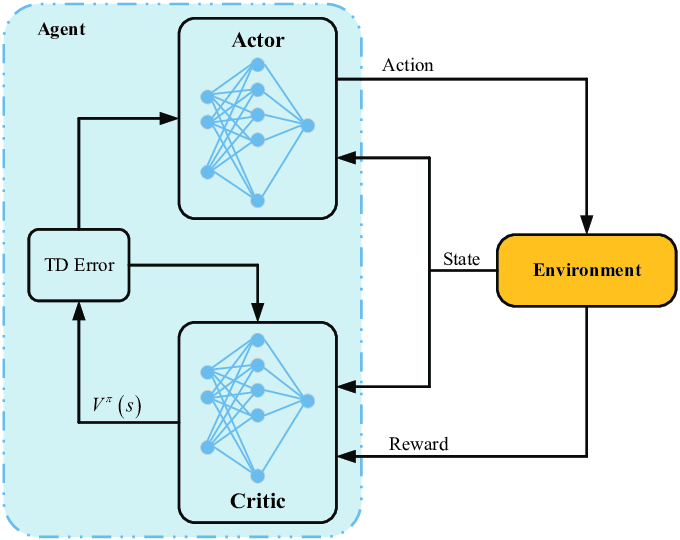
\includegraphics[height=4cm]{img/actor-critic.png}
				\end{figure}
		\end{column}
	\end{columns}
\end{frame}

\begin{frame}{On Actor-Critic: MARL settings}
	\begin{alertblock}{Idea}
		\begin{itemize}
			\item The Actor is a local shared policy that takes observations as input and returns local actions
			\item The Critic instead, is placed in a central server
			\item The Critic has a global view of the system $\implies$ it could use overall state information 
			\item The Actor is then influenced by global data, but at \emph{deployment} time it does not use them
		\end{itemize}
	\end{alertblock}
	\begin{exampleblock}{Considerations}
		\begin{itemize}
			\item[{\color{teal} \faThumbsUp}] A balanced between fully decentralised and centralised method
			\item[{\color{red} \faThumbsDown}] Require simulations $\implies$ cannot be used in online systems  
		\end{itemize}
	\end{exampleblock}
\end{frame}

\begin{frame}{Handling Partial Observability}
	\begin{exampleblock}{}
		\begin{itemize}
			\item As I mentioned, CAS are partially observable \dots
			\item \dots But the methods proposed does not handle this matter in any sense
			\item Recurrent Neural Networks (i.e. Neural Networks with \emph{memory}) are an emergent trend to handle this issue
			\item In MAS settings, RNNs and Hysteretic updates are used together to handle both non-stationarity and partial observability~\footnote[frame]{\fullcite{DBLP:conf/icml/OmidshafieiPAHV17}}
			\item[{\color{red} \faThumbsDown}] It is not clear if RNNs are a solution for Partial Observability
		\end{itemize}
	\end{exampleblock}
\end{frame}

\begin{frame}{Handling large scale systems}
	\begin{exampleblock}{}
		\begin{itemize}
			\item Agent size was not a central problem in the first MARL works
			\item Independent learners are typically deployed when we have to deal with several agents \dots
			\item \dots but it makes the learning process noising
			\item Lately, a novel trend emerges to handle this problem, the so-called Mean-Field Reinforcement Learning\footnote[frame]{\fullcite{DBLP:conf/icml/YangLLZZW18}}
		\end{itemize}
	\end{exampleblock}
\end{frame}

\begin{frame}{Handling large scale systems: On Mean-Field Reinforcement Learning}
	\begin{exampleblock}{}
		\begin{itemize}
			\item The learning problem is set up as a joint action learners
			\item In Mean-Field, the system in modelled as two agent, the main agent and the rest 
			\item In Mean Field Reinforcement Learning, the rest is computed as the mean action taken by the neighbourhood
			\item[{\color{teal}\faThumbsUp}] It has theoretical guarantees
			\item[{\color{teal}\faThumbsUp}] It is easily used also in CAS
			\item[{{\color{red}\faThumbsDown}}] The approaches proposed are offline --- no online adaptation.
		\end{itemize}
	\end{exampleblock}
\end{frame}

\begin{frame}{Handling Multi-Agent credit assignment problem}
	\begin{exampleblock}{}
		\begin{itemize}
			\item In CAS settings, typically we have a global reward function
			\item[{\color{red} \faThumbsDown}] It is hard to understand the influence of the agent action on that signal
			\item This is known as Multi-Agent credit assignment problem
			\item It is tackled in COIN approach~\parencite{wolpert1999introduction} \dots
			\item \dots but it required to run several simulations to understand each agent influence
			\item COMA\footnote[frame]{\fullcite{DBLP:conf/aaai/FoersterFANW18}} is a novel approach that uses an Actor-Critic setting with a contrafacutal baseline 
		\end{itemize}
	\end{exampleblock}
\end{frame}

%\begin{frame}{Not explored issue: Global clock}
%	\begin{exampleblock}{}
%		\begin{itemize}
%			\item Works on Multi-Agent Reinforcement Learning consider Stochastic games as the model of the environment
%			\item There, agents action synchronously, i.e. at the time step t+1 all agents have done their action
%			\item This is impossible to assume in CAS
%			\item Any ideas? Lamport logical clock? 
%		\end{itemize}
%	\end{exampleblock}
%\end{frame}
%===============================================================================

%% Parla di come gestire l'osservabilità parziale
%% Parla delle tecniche Actor-Critic associate al centralised learning, decentralised execution
%% Parla di Reinforce

%===============================================================================
\section*{}
%===============================================================================

%/////////
\frame{\titlepage}
%/////////

%===============================================================================
\section*{\refname}
%===============================================================================

%%%%
\setbeamertemplate{page number in head/foot}{}
%/////////
\begin{frame}[c,noframenumbering, allowframebreaks]{\refname}
%\begin{frame}[t,allowframebreaks,noframenumbering]{\refname}
	\tiny
	\nocite{*}
	\printbibliography
\end{frame}
%/////////

%%%%%%%%%%%%%%%%%%%%%%%%%%%%%%%%%%%%%%%%%%%%%%%%%%%%%%%%%%%%%%%%%%%%%%%%%%%%%%%%
\end{document}
%%%%%%%%%%%%%%%%%%%%%%%%%%%%%%%%%%%%%%%%%%%%%%%%%%%%%%%%%%%%%%%%%%%%%%%%%%%%%%%%
